\documentclass{article}\usepackage[]{graphicx}\usepackage[]{color}
% maxwidth is the original width if it is less than linewidth
% otherwise use linewidth (to make sure the graphics do not exceed the margin)
\makeatletter
\def\maxwidth{ %
  \ifdim\Gin@nat@width>\linewidth
    \linewidth
  \else
    \Gin@nat@width
  \fi
}
\makeatother

\definecolor{fgcolor}{rgb}{0.345, 0.345, 0.345}
\newcommand{\hlnum}[1]{\textcolor[rgb]{0.686,0.059,0.569}{#1}}%
\newcommand{\hlstr}[1]{\textcolor[rgb]{0.192,0.494,0.8}{#1}}%
\newcommand{\hlcom}[1]{\textcolor[rgb]{0.678,0.584,0.686}{\textit{#1}}}%
\newcommand{\hlopt}[1]{\textcolor[rgb]{0,0,0}{#1}}%
\newcommand{\hlstd}[1]{\textcolor[rgb]{0.345,0.345,0.345}{#1}}%
\newcommand{\hlkwa}[1]{\textcolor[rgb]{0.161,0.373,0.58}{\textbf{#1}}}%
\newcommand{\hlkwb}[1]{\textcolor[rgb]{0.69,0.353,0.396}{#1}}%
\newcommand{\hlkwc}[1]{\textcolor[rgb]{0.333,0.667,0.333}{#1}}%
\newcommand{\hlkwd}[1]{\textcolor[rgb]{0.737,0.353,0.396}{\textbf{#1}}}%
\let\hlipl\hlkwb

\usepackage{framed}
\makeatletter
\newenvironment{kframe}{%
 \def\at@end@of@kframe{}%
 \ifinner\ifhmode%
  \def\at@end@of@kframe{\end{minipage}}%
  \begin{minipage}{\columnwidth}%
 \fi\fi%
 \def\FrameCommand##1{\hskip\@totalleftmargin \hskip-\fboxsep
 \colorbox{shadecolor}{##1}\hskip-\fboxsep
     % There is no \\@totalrightmargin, so:
     \hskip-\linewidth \hskip-\@totalleftmargin \hskip\columnwidth}%
 \MakeFramed {\advance\hsize-\width
   \@totalleftmargin\z@ \linewidth\hsize
   \@setminipage}}%
 {\par\unskip\endMakeFramed%
 \at@end@of@kframe}
\makeatother

\definecolor{shadecolor}{rgb}{.97, .97, .97}
\definecolor{messagecolor}{rgb}{0, 0, 0}
\definecolor{warningcolor}{rgb}{1, 0, 1}
\definecolor{errorcolor}{rgb}{1, 0, 0}
\newenvironment{knitrout}{}{} % an empty environment to be redefined in TeX

\usepackage{alltt}

\usepackage{float}

% Set the margins on the page to not be so large
\addtolength{\oddsidemargin}{-.875in}
\addtolength{\evensidemargin}{-.875in}
\addtolength{\textwidth}{1.75in}
\addtolength{\topmargin}{-.875in}
\addtolength{\textheight}{1.75in}

% Take off page numbering
\pagenumbering{gobble}
\IfFileExists{upquote.sty}{\usepackage{upquote}}{}
\begin{document}

\title{%
  1.4.2 Data Exploration Example \\
  \smallskip
  \large Stat 5100: Dr. Bean
}
\date{}

\maketitle

\textbf{Example: } Here we will do some various data manipulations and explorations in R. We will look at the ``iris'' dataset, a very famous dataset that is automatically available in R.

\begin{knitrout}
\definecolor{shadecolor}{rgb}{0.969, 0.969, 0.969}\color{fgcolor}\begin{kframe}
\begin{alltt}
\hlcom{# Look at the first 6 observations in the iris dataset:}
\hlkwd{head}\hlstd{(iris)}
\end{alltt}
\begin{verbatim}
##   Sepal.Length Sepal.Width Petal.Length Petal.Width Species
## 1          5.1         3.5          1.4         0.2  setosa
## 2          4.9         3.0          1.4         0.2  setosa
## 3          4.7         3.2          1.3         0.2  setosa
## 4          4.6         3.1          1.5         0.2  setosa
## 5          5.0         3.6          1.4         0.2  setosa
## 6          5.4         3.9          1.7         0.4  setosa
\end{verbatim}
\begin{alltt}
\hlcom{# What variables are contained in this dataset?}
\hlkwd{names}\hlstd{(iris)}
\end{alltt}
\begin{verbatim}
## [1] "Sepal.Length" "Sepal.Width"  "Petal.Length" "Petal.Width"  "Species"
\end{verbatim}
\begin{alltt}
\hlcom{# What variable types are the columns?}
\hlkwd{str}\hlstd{(iris)}
\end{alltt}
\begin{verbatim}
## 'data.frame':	150 obs. of  5 variables:
##  $ Sepal.Length: num  5.1 4.9 4.7 4.6 5 5.4 4.6 5 4.4 4.9 ...
##  $ Sepal.Width : num  3.5 3 3.2 3.1 3.6 3.9 3.4 3.4 2.9 3.1 ...
##  $ Petal.Length: num  1.4 1.4 1.3 1.5 1.4 1.7 1.4 1.5 1.4 1.5 ...
##  $ Petal.Width : num  0.2 0.2 0.2 0.2 0.2 0.4 0.3 0.2 0.2 0.1 ...
##  $ Species     : Factor w/ 3 levels "setosa","versicolor",..: 1 1 1 1 1 1 1 1 1 1 ...
\end{verbatim}
\begin{alltt}
\hlcom{# How many observations (rows) does the dataset have?}
\hlkwd{nrow}\hlstd{(iris)}
\end{alltt}
\begin{verbatim}
## [1] 150
\end{verbatim}
\end{kframe}
\end{knitrout}

Now, let's create some graphics to explore this dataset a bit more:

\begin{knitrout}
\definecolor{shadecolor}{rgb}{0.969, 0.969, 0.969}\color{fgcolor}\begin{kframe}
\begin{alltt}
\hlcom{# Create a scatterplot of sepal width and petal width}
\hlkwd{plot}\hlstd{(iris}\hlopt{$}\hlstd{Sepal.Width, iris}\hlopt{$}\hlstd{Petal.Width,} \hlkwc{main} \hlstd{=} \hlstr{"Scatterplot of sepal and petal width"}\hlstd{,}
     \hlkwc{xlab} \hlstd{=} \hlstr{"Sepal Width"}\hlstd{,} \hlkwc{ylab} \hlstd{=} \hlstr{"Petal Width"}\hlstd{)}
\end{alltt}
\end{kframe}

{\centering 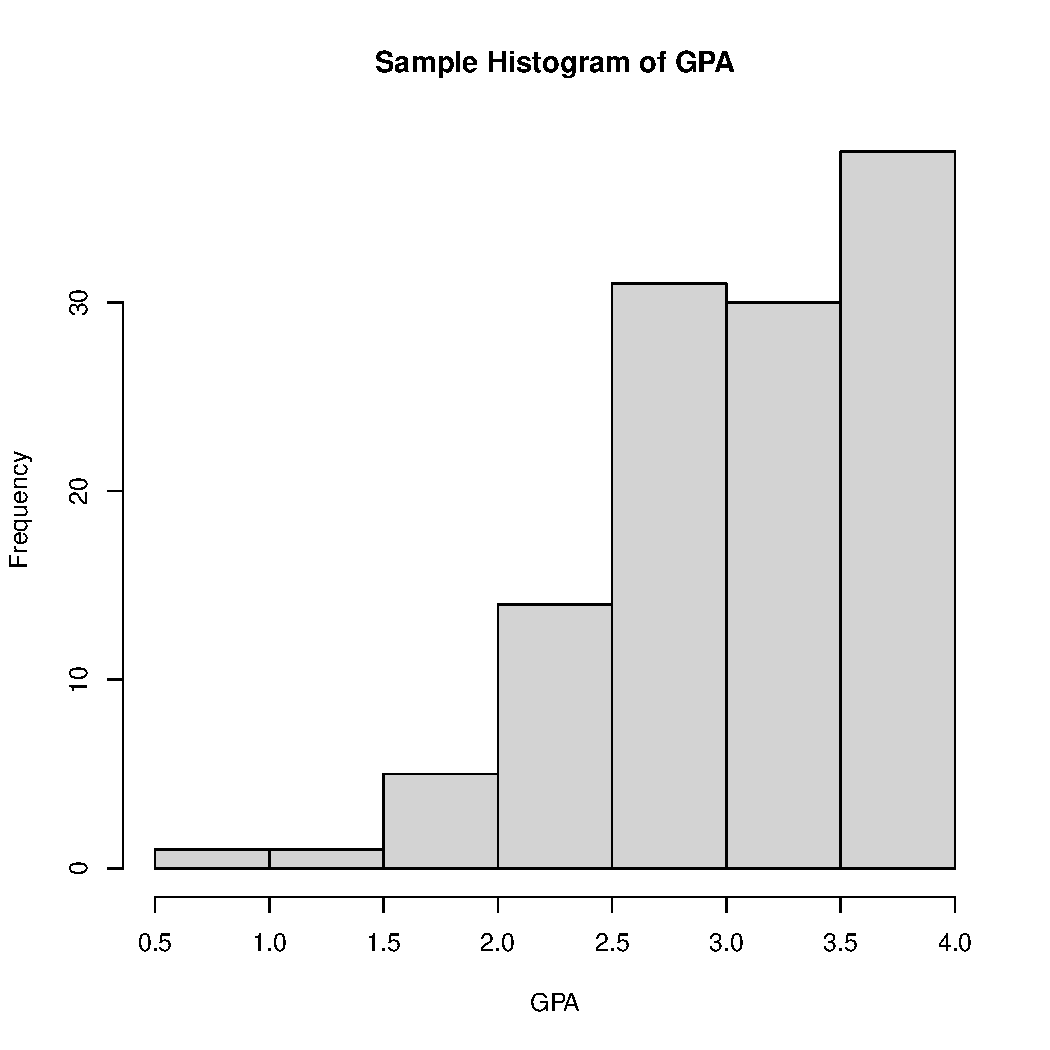
\includegraphics[width=0.6\textwidth]{figure/unnamed-chunk-2-1} 

}


\begin{kframe}\begin{alltt}
\hlcom{# Create a box plot of petal width}
\hlkwd{boxplot}\hlstd{(iris}\hlopt{$}\hlstd{Petal.Width,} \hlkwc{ylab} \hlstd{=} \hlstr{"Petal Width"}\hlstd{)}
\end{alltt}
\end{kframe}

{\centering 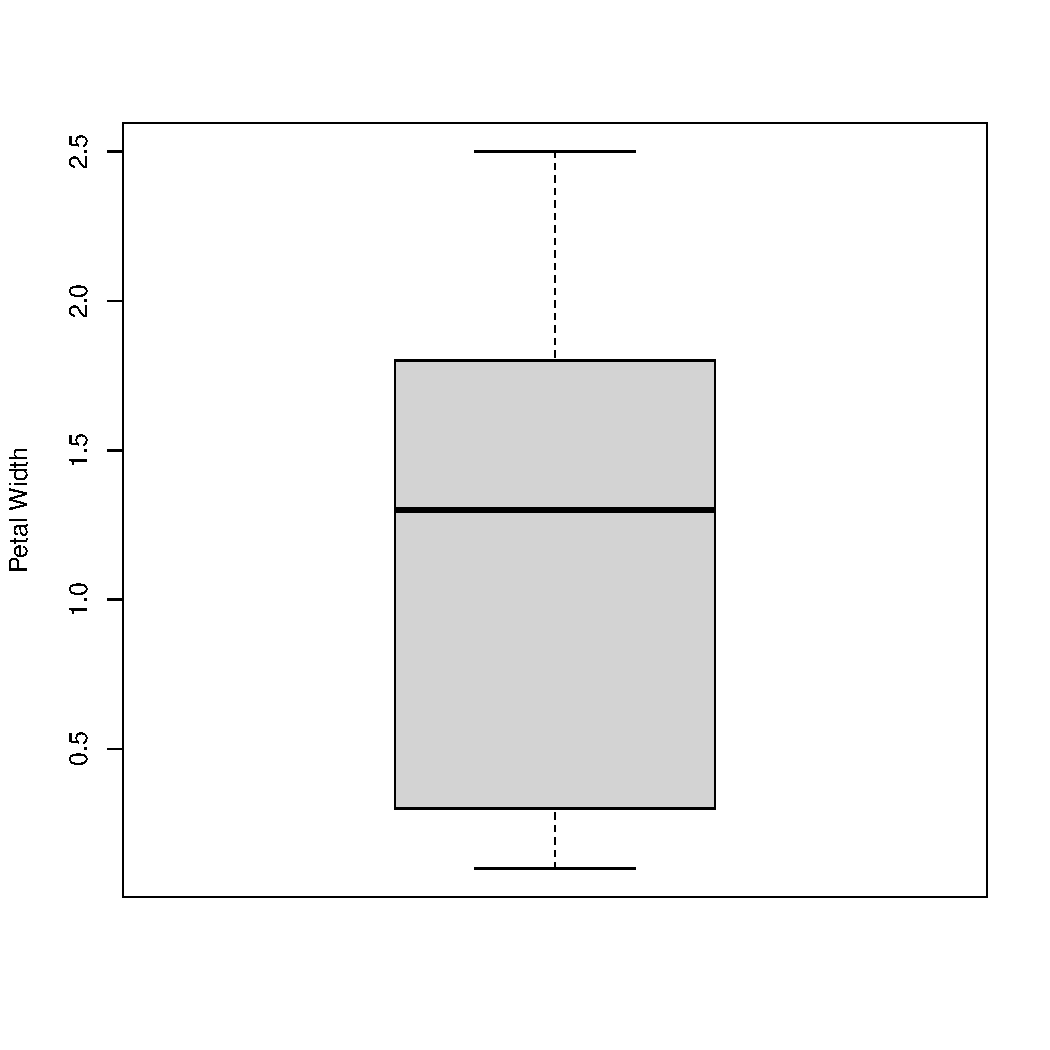
\includegraphics[width=0.6\textwidth]{figure/unnamed-chunk-2-2} 

}


\begin{kframe}\begin{alltt}
\hlcom{# How normally distributed is the sepal length variable? Create both a}
\hlcom{# histogram and a Q-Q plot to check.}
\hlkwd{hist}\hlstd{(iris}\hlopt{$}\hlstd{Sepal.Length,} \hlkwc{main} \hlstd{=} \hlstr{"Histogram of Sepal Length"}\hlstd{,} \hlkwc{xlab} \hlstd{=} \hlstr{"Sepal Length"}\hlstd{)}
\end{alltt}
\end{kframe}

{\centering 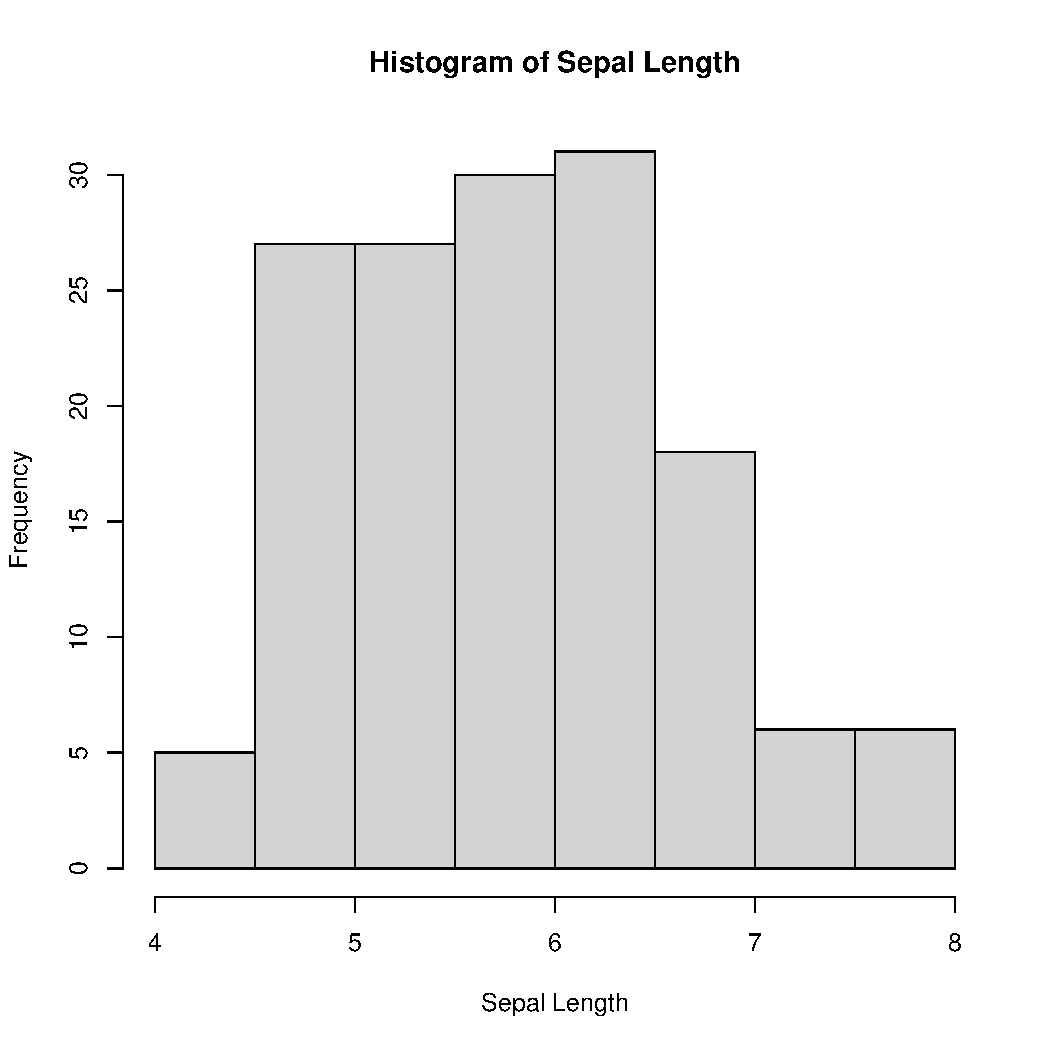
\includegraphics[width=0.6\textwidth]{figure/unnamed-chunk-2-3} 

}


\begin{kframe}\begin{alltt}
\hlkwd{qqnorm}\hlstd{(iris}\hlopt{$}\hlstd{Sepal.Length,} \hlkwc{main} \hlstd{=} \hlstr{"Q-Q plot to check normality"}\hlstd{)}
\hlkwd{qqline}\hlstd{(iris}\hlopt{$}\hlstd{Sepal.Length)}
\end{alltt}
\end{kframe}

{\centering 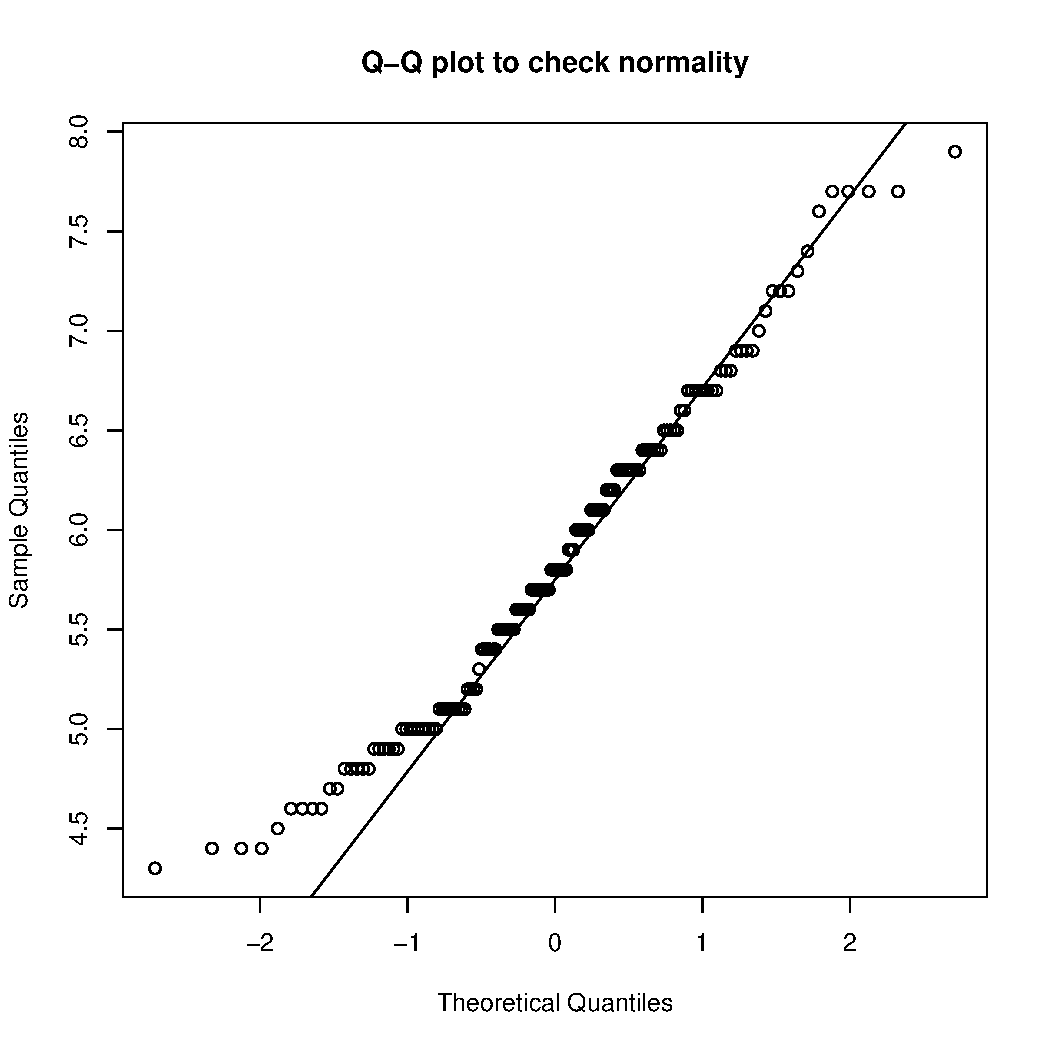
\includegraphics[width=0.6\textwidth]{figure/unnamed-chunk-2-4} 

}



\end{knitrout}

Let's create a linear model where we predict sepal length from sepal width.

\begin{knitrout}
\definecolor{shadecolor}{rgb}{0.969, 0.969, 0.969}\color{fgcolor}\begin{kframe}
\begin{alltt}
\hlstd{iris_lm} \hlkwb{<-} \hlkwd{lm}\hlstd{(Petal.Length} \hlopt{~} \hlstd{Petal.Width,} \hlkwc{data} \hlstd{= iris)}

\hlstd{stat5100}\hlopt{::}\hlkwd{fit_plot}\hlstd{(iris_lm,} \hlkwc{main} \hlstd{=} \hlstr{"Fit plot"}\hlstd{,} \hlkwc{xlab} \hlstd{=} \hlstr{"Petal Width"}\hlstd{,}
                   \hlkwc{ylab} \hlstd{=} \hlstr{"Petal Length"}\hlstd{)}
\end{alltt}
\end{kframe}

{\centering 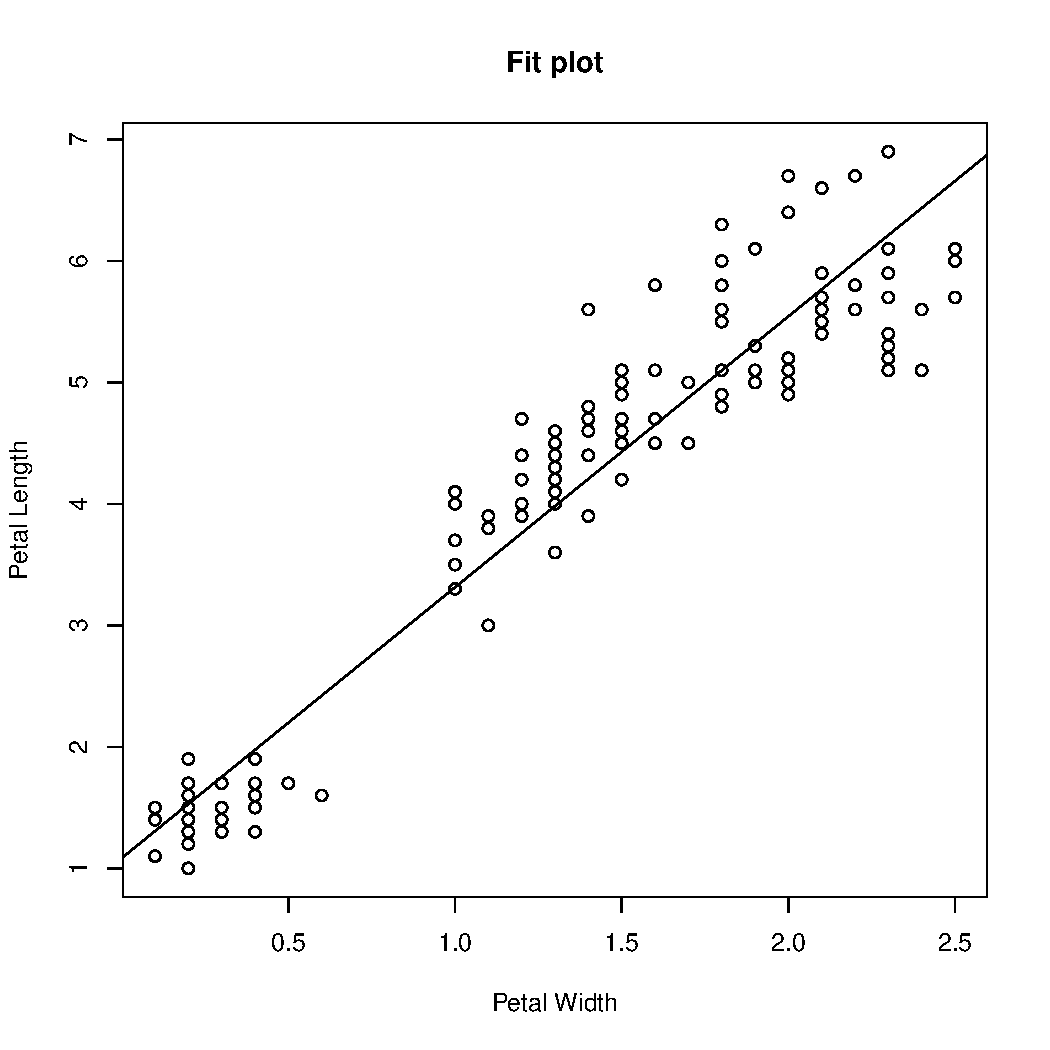
\includegraphics[width=0.6\textwidth]{figure/unnamed-chunk-3-1} 

}



\end{knitrout}

What if we want to make a prediction using our linear model? Suppose that we have two flowers with petal widths of 0.3 and 2.4.

\begin{knitrout}
\definecolor{shadecolor}{rgb}{0.969, 0.969, 0.969}\color{fgcolor}\begin{kframe}
\begin{alltt}
\hlstd{my_beautiful_two_flowers} \hlkwb{<-} \hlkwd{data.frame}\hlstd{(}\hlkwc{Petal.Width} \hlstd{=} \hlkwd{c}\hlstd{(}\hlnum{0.3}\hlstd{,} \hlnum{2.4}\hlstd{))}

\hlstd{predicted_petal_length} \hlkwb{<-} \hlkwd{predict}\hlstd{(iris_lm, my_beautiful_two_flowers)}
\hlstd{predicted_petal_length}
\end{alltt}
\begin{verbatim}
##        1        2 
## 1.752540 6.435415
\end{verbatim}
\end{kframe}
\end{knitrout}

Based upon the above, for the flower with the petal width of 0.3 cm we would predict that the length is 1.75 cm and for the petal width of 2.4 cm we would predict that the length is 6.44 cm.

\end{document}
